% =====================================================================
% 강의 노트: Gelman, Hill, & Yajima (2012)
%   "Why We (Usually) Don't Have to Worry About Multiple Comparisons"
% =====================================================================
% Compile with:  xelatex lecture_notes.tex  (twice for cross-refs)
% Fonts: Noto Sans KR (Hangul + Hanja); install once with:
%   curl -L -o ~/.fonts/NotoSansKR-Regular.otf <google fonts url>
% =====================================================================
\documentclass[11pt,a4paper]{article}

\usepackage{fontspec}
\setmainfont[BoldFont={Noto Sans KR Bold}]{Noto Sans KR}
\setsansfont[BoldFont={Noto Sans KR Bold}]{Noto Sans KR}
\setmonofont{Latin Modern Mono}

\usepackage[margin=1in]{geometry}
\usepackage{amsmath,amssymb,bm}
\usepackage{graphicx}
\usepackage{booktabs}
\usepackage{hyperref}
\usepackage{xcolor}
\usepackage{tcolorbox}
\tcbuselibrary{breakable,skins}
\usepackage{caption}
\captionsetup{font=small,labelfont=bf}
\usepackage{enumitem}
\setlist{itemsep=2pt,topsep=4pt}

\hypersetup{colorlinks=true, linkcolor=blue!60!black,
            urlcolor=blue!60!black, citecolor=blue!60!black}

\newcommand{\E}{\mathbb{E}}
\newcommand{\Var}{\mathrm{Var}}
\newcommand{\Normal}{\mathcal{N}}

\newtcolorbox{keyidea}[1][]{colback=blue!5,colframe=blue!50!black,
  fonttitle=\bfseries, title=핵심 아이디어, breakable,#1}
\newtcolorbox{warn}[1][]{colback=red!5,colframe=red!60!black,
  fonttitle=\bfseries, title=빈도주의가 자주 빠지는 함정, breakable,#1}
\newtcolorbox{exercise}[1][]{colback=gray!5,colframe=gray!50!black,
  fonttitle=\bfseries, title=연습문제, breakable,#1}
\newtcolorbox{termbox}[1][]{colback=yellow!8,colframe=orange!70!black,
  fonttitle=\bfseries, title=용어 안내, breakable,#1}

\title{
  \LARGE 다회검정 문제와 다층모형 \\[4pt]
  \large Why We (Usually) Don't Have to Worry About Multiple Comparisons \\[2pt]
  \small Gelman, Hill, \& Yajima (2012) \\
  \emph{Journal of Research on Educational Effectiveness}, 5: 189--211
}
\author{강의 노트}
\date{}

\begin{document}
\maketitle

\begin{termbox}
본 강의자료에서는 \textbf{다회검정 (multiple comparisons; 多回檢定)} 을 표준 용어로 사용한다.
한국 통계학회에서 통용되는 \textbf{``다중비교''} 또한 같은 의미로 사용되는 용어이며, 두 표현은 본 자료에서 동의어로 취급한다.

\smallskip
\textbf{왜 ``다회검정''인가?}\quad 문제의 본질은 \emph{하나의 데이터셋(또는 하나의 연구)에 대해 검정을 여러 번 반복하기 때문에 누적 오류율이 부풀어 오른다}는 것이다.
한자 ``다중(多重)''의 ``겹쳐 누적된''이라는 뜻은 이 현상을 잘 잡지 못한다 --- 빈도주의 검정들은 서로 겹치는 것이 아니라 단순히 \emph{여러 번} 수행될 뿐이다.
이에 비해 ``다회(多回)''의 ``여러 차례''라는 뜻이 본질을 더 정확히 포착한다.
다만 ``다중비교''/``다중검정''이 학계에서 표준 용어로 굳어져 있으므로, 학생들은 두 표현 모두에 익숙해질 필요가 있다.
\end{termbox}

\tableofcontents
\vspace{1em}
\hrule
\vspace{1em}

% =====================================================================
\section{왜 이 논문을 읽어야 하는가}

수많은 가설을 한꺼번에 검정하는 상황은 거의 모든 응용 통계에서 나타난다.
8개 학교에서의 처치 효과, 50개 주의 평균 점수, 1{,}000명의 교사 효과, 100개 유전자의 발현 차이 등.

전통적인 빈도주의 해법은 \textbf{p-value를 조정}하는 것이다.
\begin{itemize}
  \item Bonferroni: $\alpha' = \alpha / k$
  \item Sidak: $\alpha' = 1 - (1-\alpha)^{1/k}$
  \item Benjamini--Hochberg (FDR)
\end{itemize}
이 모든 방법은 \emph{Type 1 error}, 즉 ``실제로는 효과가 없는데 있다고 잘못 결론짓는 비율''을 통제하는 데 초점이 맞춰져 있다.

\begin{keyidea}
Gelman 등은 다음과 같이 주장한다:
\begin{enumerate}
  \item Type 1 error는 \emph{진짜 효과가 정확히 0}이라는 가정 위에 서 있다.
        사회과학·교육학·정책평가에서 이 가정은 거의 항상 \textbf{틀렸다}.
  \item 진짜 걱정해야 할 것은 \textbf{Type S} (sign --- 부호를 거꾸로 추정) 과 \textbf{Type M} (magnitude --- 효과 크기를 과대 추정) 오류이다.
  \item 이 모든 문제는 \emph{베이지안 다층(hierarchical) 모형}으로 자연스럽게 다룰 수 있다.
        Bonferroni처럼 신뢰구간을 인위적으로 \emph{넓히는} 대신, 다층모형은 추정치들을 서로 \emph{끌어당긴다(shrinkage)}.
\end{enumerate}
\end{keyidea}

% =====================================================================
\section{빈도주의 관점에서 본 다회검정 문제 (IHDP 8개 사이트)}

\subsection{데이터와 모형}

Infant Health and Development Program (IHDP)는 미국 8개 사이트에서 저체중·미숙아에게 가정방문과 양질의 보육 서비스를 제공한 무작위 통제 실험이다.
각 사이트별로 처치 효과가 동일한지 다른지를 알고 싶다.

학생 $i$의 검사 점수 $y_i$를 다음과 같이 모형화한다:
\begin{equation}
\label{eq:classical}
  y_i = \sum_{j=1}^{8}\bigl(\gamma_j S_i^j + \delta_j S_i^j P_i\bigr) + \varepsilon_i,
  \quad \varepsilon_i \sim \Normal(0,\sigma^2)
\end{equation}
여기서 $S_i^j$는 사이트 $j$에 속하는지를 가리키는 더미, $P_i$는 처치 여부(0/1), $\gamma_j$는 사이트 $j$의 통제군 평균, $\delta_j$는 사이트 $j$의 처치 효과이다.

\subsection{사이트별 개별 검정}

가설 $H_0^j: \delta_j = 0$을 $j=1,\dots,8$에 대해 각각 검정한다.
유의수준 $\alpha=0.05$일 때 독립을 가정하면, 8번 검정 중 적어도 1번이 $H_0$을 잘못 기각할 확률은
\[ 1 - (1-0.05)^8 \approx 0.34. \]
이것이 \textbf{family-wise error rate (FWER)} 가 부풀어 오르는 문제이다.

\subsection{Bonferroni 보정}

각 검정의 임계값을 $\alpha/k = 0.05/8 \approx 0.00625$로 낮춘다.
등가적으로 신뢰구간의 폭을 $z_{1-\alpha/(2k)} \approx 2.73$으로 \emph{넓힌다} (기존 1.96 대비).

\begin{warn}
Bonferroni는 Type 1 error를 직접 통제하지만, 그 대가로 \emph{Type 2 error}(power 손실)가 크게 증가한다.
표본 크기가 작거나 효과가 작은 사이트는 진짜 효과가 있어도 발견할 수 없게 된다.
\end{warn}

\subsection{FDR (Benjamini--Hochberg)}

``기각된 가설들 중 잘못 기각된 비율''(false discovery rate)을 통제하는 방법.
유전체학 등에서 유용하지만, 사회과학에서는 여전히 ``효과가 정확히 0''이라는 출발점에 의존하므로 한계가 있다.

% =====================================================================
\section{다른 관점: Type S, Type M error}

Gelman \& Tuerlinckx (2000)은 Type 1 / Type 2 대신 다음을 제안한다:
\begin{itemize}
  \item \textbf{Type S (sign) error}: 진짜 효과가 양수인데 ``음의 효과가 있다''고 결론.
  \item \textbf{Type M (magnitude) error}: 진짜 효과가 작은데, 유의한 추정치는 진짜 효과의 몇 배 크기로 부풀려진다.
\end{itemize}
낮은 power(큰 SE)일수록 ``유의''로 살아남은 결과는 더 극단적인 값일 수밖에 없다 --- 이른바 \emph{statistical significance filter}.

\begin{figure}[ht]
  \centering
  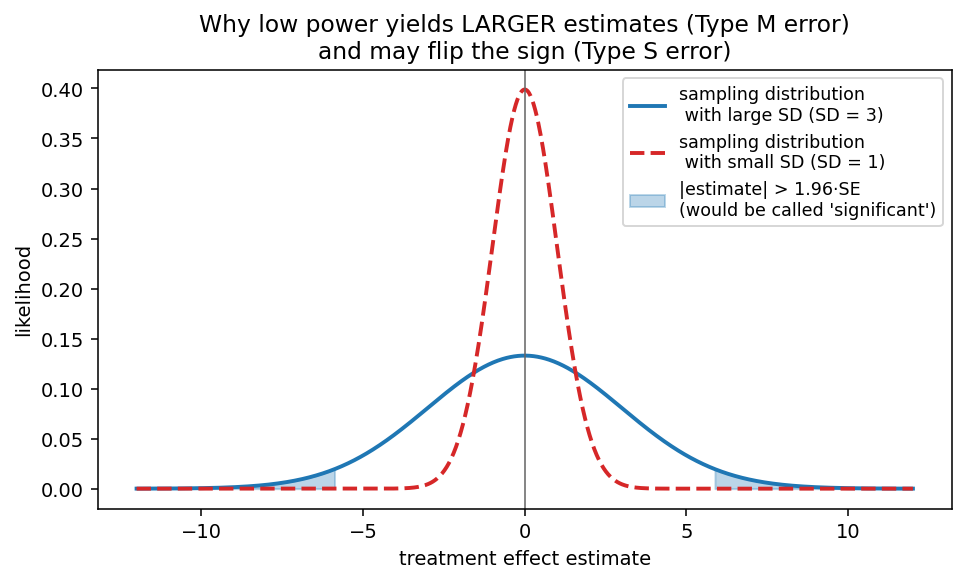
\includegraphics[width=0.85\linewidth]{../figures/fig_type_sm_intuition.png}
  \caption{두 sampling distribution. 진짜 효과가 0인데도, SE가 큰 경우(파란 곡선) ``유의''로 판정되는 결과는 진짜 효과로부터 크게 떨어진 값일 가능성이 높다.}
\end{figure}

\begin{figure}[ht]
  \centering
  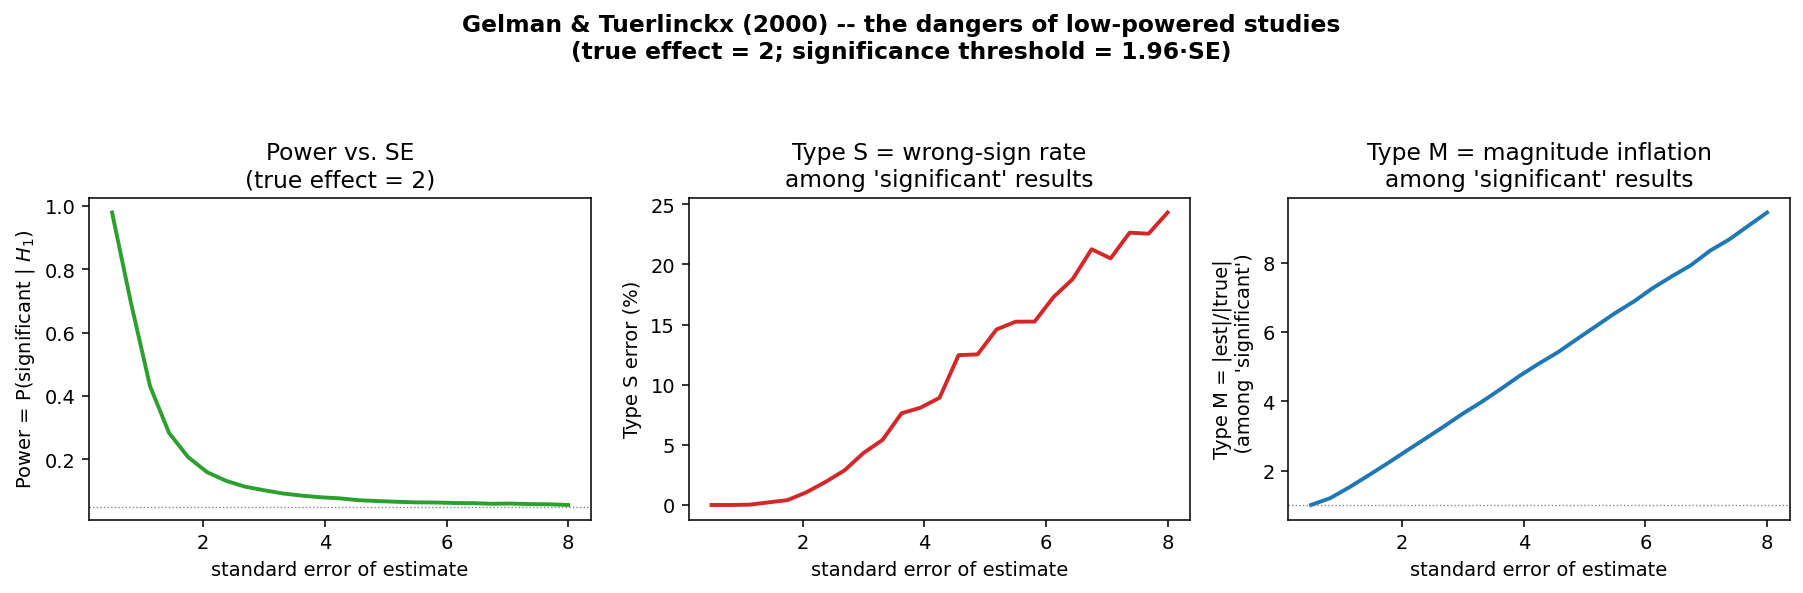
\includegraphics[width=\linewidth]{../figures/fig_type_sm_simulation.png}
  \caption{시뮬레이션: 진짜 효과 = 2일 때 SE의 함수로 본 power, Type S, Type M. SE가 커질수록 Type S/M 모두 폭증한다.}
\end{figure}

\begin{warn}
\textbf{빈도주의가 자주 하는 결정적 실수} \\
``유의하면 효과가 있는 것이고, 유의하지 않으면 효과가 없는 것이다.'' --- 이것은 \emph{틀린} 명제다.
저전력 연구에서 ``유의함''은 그 자체로 \textbf{과대 추정의 증거}이며, ``유의하지 않음''은 \textbf{정보 부족의 증거}일 뿐이다.
\end{warn}

% =====================================================================
\section{베이지안 다층(Hierarchical) 모형}
\label{sec:hierarchical}

\subsection{모형 정의}

이제 식 \eqref{eq:classical}을 다음과 같이 확장한다:
\begin{align}
  y_i      &\sim \Normal(\gamma_{j[i]} + \delta_{j[i]} P_i, \sigma_y^2) \\
  \gamma_j &\sim \Normal(\mu_\gamma, \sigma_\gamma^2) \\
  \delta_j &\sim \Normal(\mu_\delta, \sigma_\delta^2)  \quad \leftarrow \text{핵심}
\end{align}
\textbf{이 한 줄이 모든 것을 바꾼다.}
사이트별 처치 효과 $\delta_j$를 서로 독립이 아닌, \emph{공통의 분포에서 나온 값들}로 본다.
$\sigma_\delta$가 작을수록 ``사이트들의 효과는 사실 비슷하다''는 뜻이고, 큰 값일수록 ``사이트별로 효과가 매우 다르다''는 뜻이다.

\subsection{Pooling의 세 가지 양상}

\begin{itemize}
  \item \textbf{Complete pooling}: 모든 $\delta_j = \delta$ ($\sigma_\delta \to 0$의 극한)
  \item \textbf{No pooling}: 사이트별로 독립적 추정 ($\sigma_\delta \to \infty$의 극한; 빈도주의의 출발점)
  \item \textbf{Partial pooling}: 둘 사이의 데이터-주도 절충. $\sigma_\delta$를 데이터에서 추정.
\end{itemize}

\subsection{Shrinkage의 대수적 유도}

가장 간단한 정규-정규 hierarchical model:
\[
  \bar y_j \mid \theta_j \sim \Normal(\theta_j, \sigma_{\bar y}^2),
  \quad \theta_j \sim \Normal(\mu, \sigma_\theta^2).
\]
$\mu, \sigma_\theta$가 알려져 있을 때, $\theta_j$의 사후분포는 (conjugate)
\begin{align}
  \E[\theta_j \mid \bar y_j] &= w_j\, \bar y_j + (1-w_j)\,\mu, \\
  \Var(\theta_j \mid \bar y_j) &= \tfrac{1}{1/\sigma_\theta^2+1/\sigma_{\bar y}^2}, \\
  w_j &= \tfrac{\sigma_\theta^2}{\sigma_\theta^2 + \sigma_{\bar y}^2}\quad\text{(shrinkage weight)}.
\end{align}

\begin{itemize}
  \item $\sigma_{\bar y}^2 \ll \sigma_\theta^2$: $w_j \to 1$, ``개별 추정 거의 그대로 신뢰''.
  \item $\sigma_{\bar y}^2 \gg \sigma_\theta^2$: $w_j \to 0$, ``공통 평균 $\mu$로 강하게 끌어당김''.
\end{itemize}

두 그룹 차이 $\theta_j - \theta_k$의 z-score:
\begin{equation}
  z_{\mathrm{MLM}} = \underbrace{\tfrac{\bar y_j - \bar y_k}{\sqrt{2}\,\sigma_{\bar y}}}_{z_{\mathrm{classical}}}
                    \cdot \tfrac{1}{\sqrt{1 + \sigma_{\bar y}^2/\sigma_\theta^2}}.
\end{equation}
두 번째 인자는 항상 1 이하이고, $\sigma_\theta \to 0$이면 0이 된다.

\begin{figure}[ht]
  \centering
  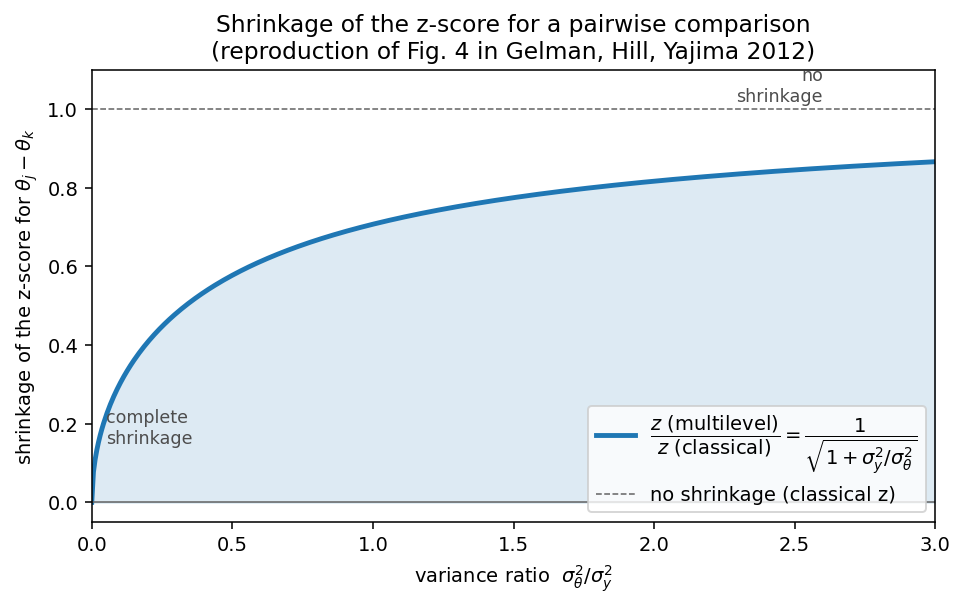
\includegraphics[width=0.7\linewidth]{../figures/fig_shrinkage_zscore.png}
  \caption{z-score의 shrinkage 양 (논문 Figure 4 재현).}
\end{figure}

\begin{keyidea}
다층모형은 ``\emph{얼마나 다회검정을 보정해야 하는가?}'' 라는 질문에 \textbf{데이터가 직접 답하도록 한다}.
$\sigma_\delta$를 데이터에서 추정하여, ``그룹들이 사실 비슷하다''면 자동으로 강한 shrinkage를 적용한다.
별도의 ad-hoc p-value 조작은 필요 없다.
\end{keyidea}

% =====================================================================
\section{예제 1: Eight Schools (Rubin 1981)}

\subsection{실제 데이터}

뉴저지의 8개 고등학교에서 진행된 SAT-Verbal 코칭 효과 메타분석.

\begin{center}
\begin{tabular}{ccc cc}
\toprule
\textbf{School} & $\bm{y_j}$ (point est.) & $\bm{\sigma_j}$ (SE) &
\textbf{Bayes M} & \textbf{Bayes SD} \\
\midrule
A & 28 & 15 & 11 & 8 \\
B &  8 & 10 &  7 & 6 \\
C & -3 & 16 &  6 & 8 \\
D &  7 & 11 &  7 & 7 \\
E & -1 &  9 &  5 & 6 \\
F &  1 & 11 &  6 & 7 \\
G & 18 & 10 & 10 & 7 \\
H & 12 & 18 &  8 & 8 \\
\bottomrule
\end{tabular}
\end{center}
(원 논문 Table 1. 첫 두 열은 원자료, 마지막 두 열은 베이지안 사후 평균/SD.)

\subsection{세 가지 분석의 비교}

\begin{figure}[ht]
  \centering
  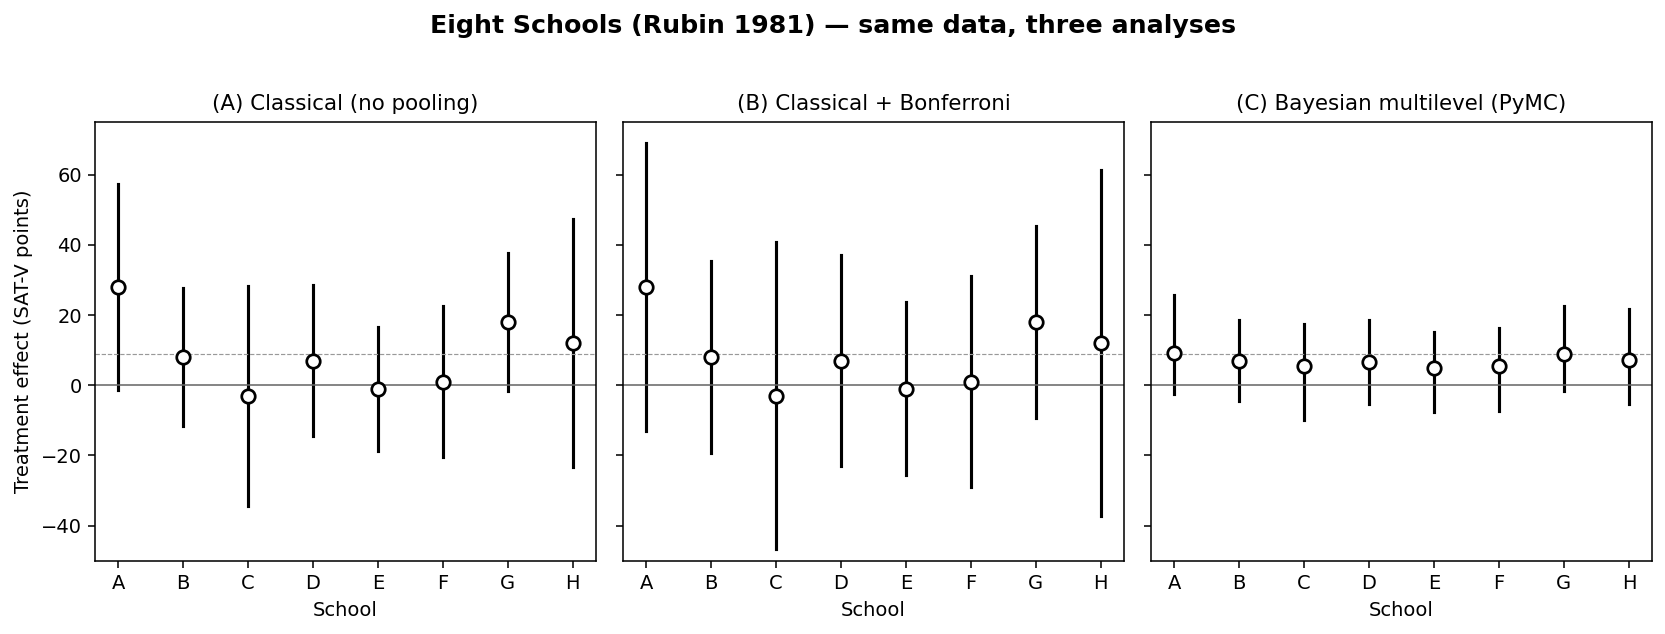
\includegraphics[width=\linewidth]{../figures/fig_eight_schools_compare.png}
  \caption{Eight Schools의 세 가지 분석. (A) 사이트별 95\% CI, (B) Bonferroni 보정, (C) 베이지안 다층모형. 학교 A (28)와 학교 C ($-3$)는 사후 평균이 각각 11과 6으로 가까워졌다.}
\end{figure}

\begin{figure}[ht]
  \centering
  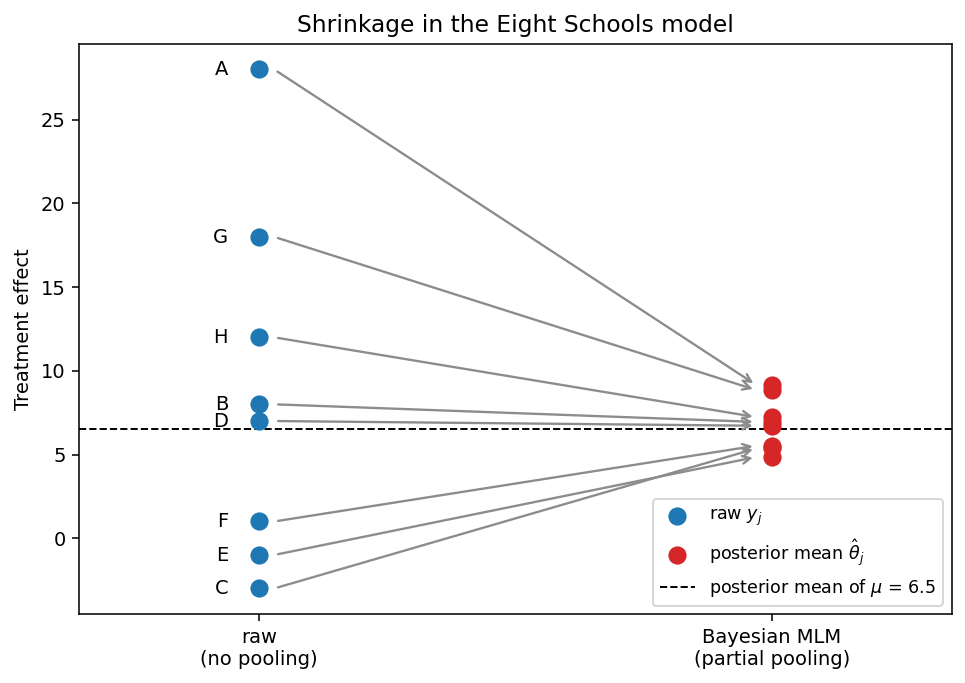
\includegraphics[width=0.7\linewidth]{../figures/fig_eight_schools_shrinkage.png}
  \caption{각 학교에 대해 raw 추정치 $y_j$ (왼쪽) 에서 사후 평균 $\hat\theta_j$ (오른쪽) 로 향하는 화살표. 평균에서 멀리 떨어진 학교일수록 더 많이 끌려간다.}
\end{figure}

\begin{figure}[ht]
  \centering
  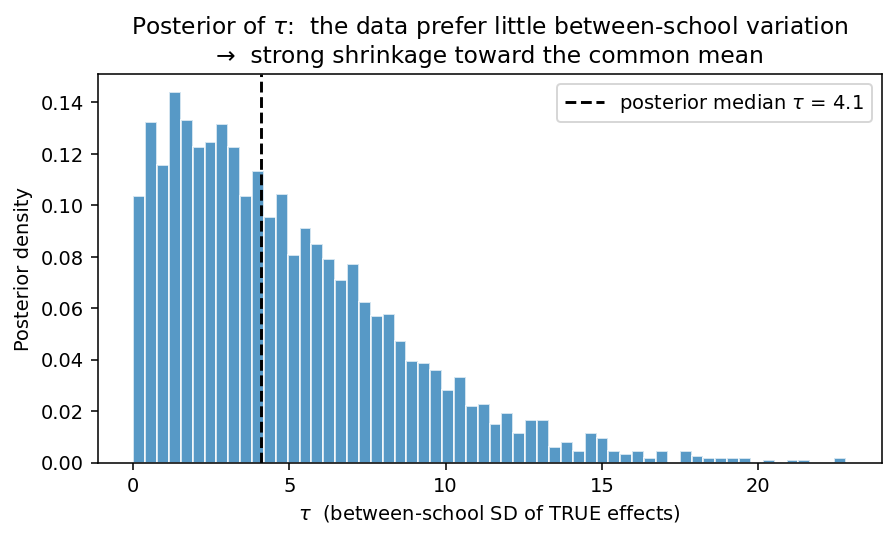
\includegraphics[width=0.6\linewidth]{../figures/fig_eight_schools_tau_posterior.png}
  \caption{학교 간 진짜 효과의 SD $\tau$에 대한 사후분포. 0 부근에 상당한 질량이 있다.}
\end{figure}

\subsection{Stan 모형 코드 (주력 MCMC 도구)}

본 강의의 주력 MCMC 샘플러는 \textbf{Stan (cmdstanpy)}이다. 비중심 매개변수화 (non-centered parameterization)를 사용해 $\tau$가 작을 때 funnel 병리를 피한다.

\begin{tcolorbox}[colback=gray!3,colframe=gray!50,title={\texttt{eight\_schools\_nc.stan}}]
\small
\begin{verbatim}
data {
  int<lower=1> J;
  vector[J]     y;
  vector<lower=0>[J] sigma;
}
parameters {
  real mu;
  real<lower=0> tau;
  vector[J] eta;
}
transformed parameters {
  vector[J] theta = mu + tau * eta;
}
model {
  mu  ~ normal(0, 10);
  tau ~ normal(0, 10);
  eta ~ std_normal();
  y   ~ normal(theta, sigma);
}
\end{verbatim}
\end{tcolorbox}

\subsection{NumPyro 버전 (보조 도구)}

같은 모형을 NumPyro로 표현하면 다음과 같다. JAX 기반의 빠른 NUTS이며, C++ 툴체인이 필요 없다.

\begin{tcolorbox}[colback=gray!3,colframe=gray!50,title={\texttt{01\_eight\_schools\_numpyro.py} (발췌)}]
\small
\begin{verbatim}
def eight_schools_model(sigma, y=None):
    mu  = numpyro.sample("mu",  dist.Normal(0., 10.))
    tau = numpyro.sample("tau", dist.HalfNormal(10.))
    with numpyro.plate("school", J):
        eta   = numpyro.sample("eta", dist.Normal(0., 1.))
        theta = numpyro.deterministic("theta", mu + tau*eta)
        numpyro.sample("y", dist.Normal(theta, sigma), obs=y)

kernel = NUTS(eight_schools_model, target_accept_prob=0.95)
mcmc   = MCMC(kernel, num_warmup=1000, num_samples=2000, num_chains=4)
mcmc.run(rng_key, sigma, y=y)
\end{verbatim}
\end{tcolorbox}

두 구현은 동일한 NUTS 알고리즘을 사용하며 사후분포 또한 사실상 일치한다. Stan은 사실상의 표준이고 진단/요약 도구가 풍부하다. NumPyro는 Python 환경에서 빠르고 GPU/TPU 활용이 용이하다.

% =====================================================================
\section{예제 2: IHDP 8개 사이트 시뮬레이션}

IHDP 원자료를 재배포할 수 없으므로 같은 구조의 데이터를 시뮬레이션한다.
사이트 8개, 사이트당 학생 80명, 진짜 효과의 평균 8.0, 사이트 간 SD 1.2.

\begin{figure}[ht]
  \centering
  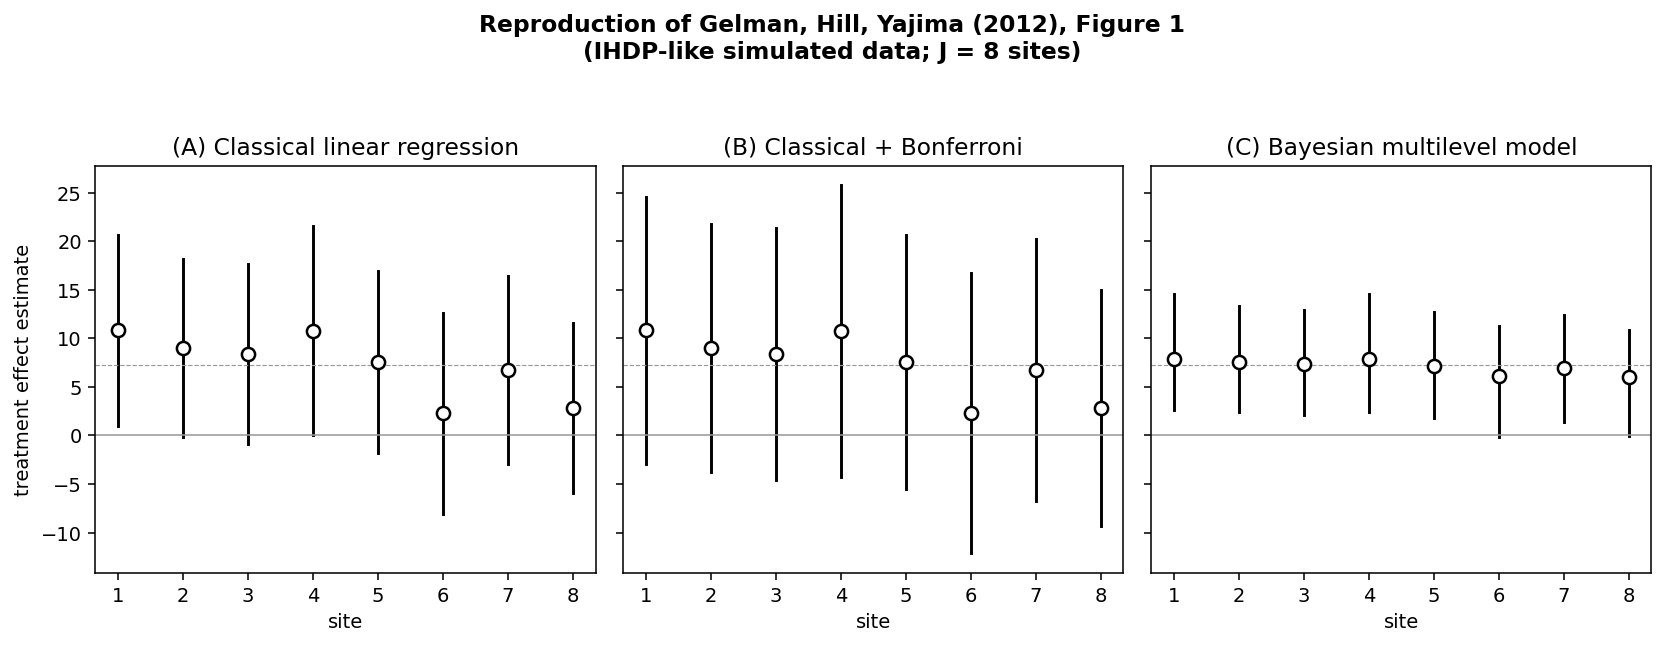
\includegraphics[width=\linewidth]{../figures/fig_ihdp_three_panels.png}
  \caption{IHDP 시뮬레이션의 세 패널 (논문 Figure 1 재현). (A) 사이트별 OLS, (B) Bonferroni, (C) Stan 다층모형. 다층모형이 점 추정치 자체를 공통 평균 부근으로 끌어당겨 안정적인 결론을 준다.}
\end{figure}

\begin{figure}[ht]
  \centering
  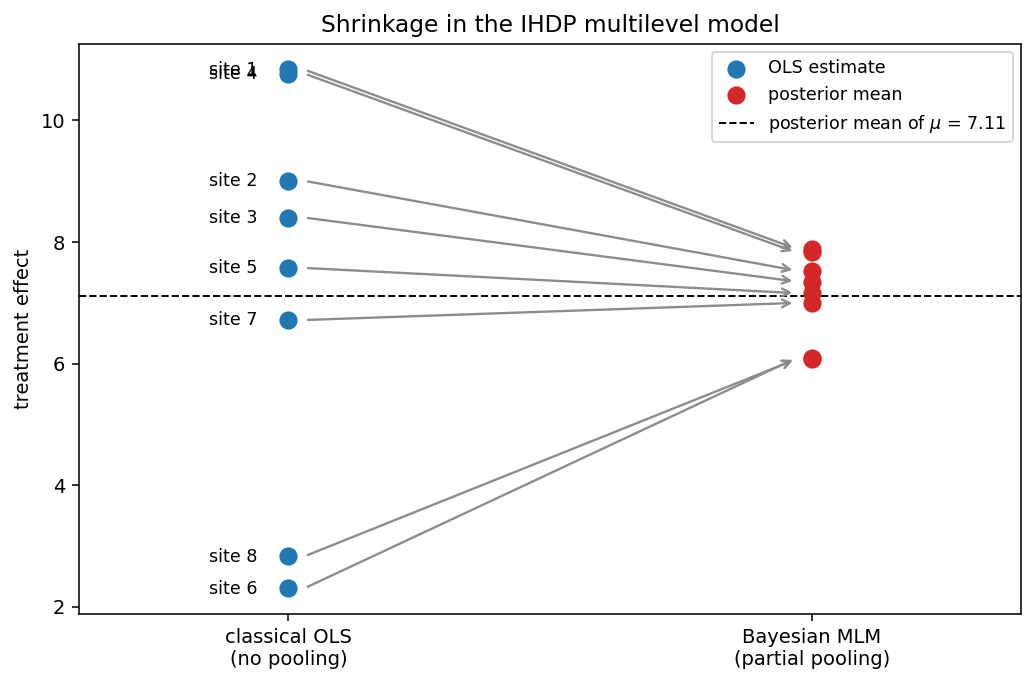
\includegraphics[width=0.85\linewidth]{../figures/fig_ihdp_shrinkage.png}
  \caption{IHDP 시뮬레이션에서 각 사이트의 raw OLS 추정치(왼쪽)와 Stan 사후 평균(오른쪽).}
\end{figure}

\subsection{Stan 모형 코드}

\begin{tcolorbox}[colback=gray!3,colframe=gray!50,title={\texttt{ihdp\_multilevel.stan} (핵심)}]
\small
\begin{verbatim}
data {
  int<lower=1> N;
  int<lower=1> J;
  array[N] int<lower=1, upper=J> site;
  vector[N] P;
  vector[N] y;
}
parameters {
  real mu_gamma, mu_delta;
  real<lower=0> sigma_gamma, sigma_delta, sigma_y;
  vector[J] gamma_raw, delta_raw;
}
transformed parameters {
  vector[J] gamma = mu_gamma + sigma_gamma * gamma_raw;
  vector[J] delta = mu_delta + sigma_delta * delta_raw;
}
model {
  // priors omitted for brevity
  vector[N] mu_i;
  for (i in 1:N) mu_i[i] = gamma[site[i]] + delta[site[i]] * P[i];
  y ~ normal(mu_i, sigma_y);
}
\end{verbatim}
\end{tcolorbox}

\begin{figure}[ht]
  \centering
  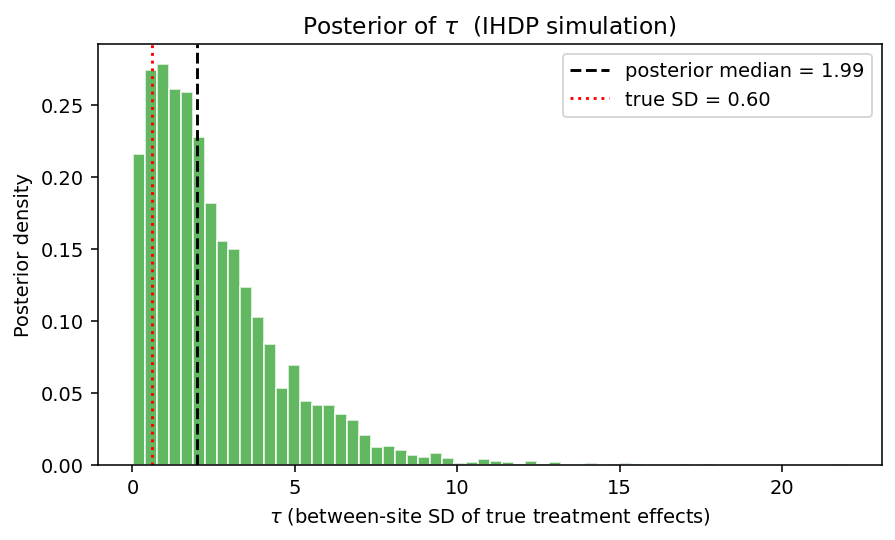
\includegraphics[width=0.6\linewidth]{../figures/fig_ihdp_tau_posterior.png}
  \caption{IHDP 시뮬레이션에서 $\sigma_\delta$의 사후분포 (Stan). 빨간 점선은 진짜 SD (1.2).}
\end{figure}

% =====================================================================
\section{결론과 권고}

\begin{keyidea}
\textbf{Gelman, Hill, \& Yajima (2012)의 메시지}
\begin{enumerate}
\item Type 1 error 패러다임은 사회과학·교육·정책 평가에서 적절한 출발점이 아니다.
\item 진짜 위험은 Type S와 Type M이며, 둘 다 저전력에서 폭증한다. Bonferroni는 power를 떨어뜨려 이 문제를 악화시킨다.
\item 다층모형은 다회검정 보정을 모델 안에 내재화한다. 그룹 간 변동 $\sigma_\delta$를 데이터에서 배우므로, 그룹들이 사실 비슷하다면 자동으로 강한 shrinkage를 적용한다.
\item Stein paradox에 의해, 다층모형의 점 추정치는 OLS보다 더 작은 MSE를 가진다.
\end{enumerate}
\end{keyidea}

\subsection{빈도주의자가 자주 하는 실수 모음}

\begin{warn}
\begin{enumerate}
\item ``8개 사이트에 8번의 t-검정을 따로 한 뒤 유의 표시.''\\
      정답: 사이트들을 함께 다층모형으로 적합.
\item ``유의하지 않으니 효과가 없다.''\\
      정답: ``유의하지 않음''은 ``SE가 컸다''는 뜻일 뿐.
\item ``유의했으니 효과가 추정값만큼 크다.''\\
      정답: 저전력 상황의 ``유의''는 거의 항상 과대 추정 (Type M).
\item ``Bonferroni를 적용하면 안전하다.''\\
      정답: Type 1만 통제. Type 2/S/M은 모두 악화.
\item ``각 그룹이 다르므로 pooling은 하면 안 된다.''\\
      정답: 다층모형은 \emph{그룹이 얼마나 다른지 자체를} 데이터에서 추정.
\end{enumerate}
\end{warn}

\subsection{언제 다층모형이 가장 유용한가}

\begin{itemize}
  \item 그룹 수 $J$가 5 이상이고 각 그룹의 데이터가 비교적 작아 잡음이 큰 경우.
  \item 그룹들이 교환 가능 (exchangeable) 하다고 볼 수 있는 경우.
  \item 그룹 수준 공변량 ($x_j$) 이 있다면 더욱 좋다 ($\delta_j \sim \Normal(\mu_0 + \beta x_j, \sigma_\delta^2)$ 로 확장).
\end{itemize}

% =====================================================================
\section{연습문제}

\begin{exercise}
\textbf{(1) 손으로 푸는 shrinkage.}
Eight Schools 데이터에서 학교 A ($y_1=28, \sigma_1=15$)와 학교 C ($y_3=-3, \sigma_3=16$)를 생각하자.
$\mu=8, \tau=5$로 고정되어 있다고 가정할 때, 각 학교의 사후 평균과 사후 표준편차를 손으로 계산하라.
\end{exercise}

\begin{exercise}
\textbf{(2) Stan vs NumPyro 비교.}
\texttt{01\_eight\_schools\_stan.py} 와 \texttt{01\_eight\_schools\_numpyro.py} 를 모두 실행하고, 사후 평균과 $\tau$의 사후 분위수가 일치하는지 비교하라.
어느 쪽이 더 빠른가? 어느 쪽이 진단 출력이 더 풍부한가?
\end{exercise}

\begin{exercise}
\textbf{(3) Bonferroni vs. shrinkage.}
\texttt{02\_ihdp\_simulation\_stan.py} 의 \texttt{n\_per\_site=80}을 \texttt{20}으로 바꿔서 다시 실행하라.
어느 분석이 더 많이 변하는가? 왜 그런가?
\end{exercise}

\begin{exercise}
\textbf{(4) Type M의 실험.}
\texttt{03\_type\_s\_m\_errors.py} 의 \texttt{true\_effect} 를 0.5, 2, 8로 바꿔가며 실행하라.
효과 크기가 클수록 Type M error는 어떻게 변하는가? 직관적으로 설명하라.
\end{exercise}

\begin{exercise}
\textbf{(5) $\tau$의 prior 의존성.}
\texttt{eight\_schools\_nc.stan} 에서 $\tau \sim \text{Half-Normal}(0,10)$ 을 $\text{Half-Cauchy}(0,5)$ 로 바꾸면 사후분포가 어떻게 달라지는가?
Gelman (2006) ``Prior distributions for variance parameters'' 을 참고하라.
\end{exercise}

\vspace{1em}
\hrule
\vspace{0.5em}
\small
\textbf{참고문헌}\\
Gelman, A., Hill, J., \& Yajima, M. (2012). Why we (usually) don't have to worry about multiple comparisons. \emph{Journal of Research on Educational Effectiveness}, 5(2), 189--211.\\
Rubin, D. B. (1981). Estimation in parallel randomized experiments. \emph{Journal of Educational Statistics}, 6, 377--401.\\
Gelman, A., \& Tuerlinckx, F. (2000). Type S error rates for classical and Bayesian single and multiple comparison procedures. \emph{Computational Statistics}, 15, 373--390.\\
Gelman (2006). Prior distributions for variance parameters in hierarchical models. \emph{Bayesian Analysis}, 1, 515--533.\\
Carpenter, B. et al. (2017). Stan: A probabilistic programming language. \emph{Journal of Statistical Software}, 76(1).\\
Phan, D., Pradhan, N., \& Jankowiak, M. (2019). Composable effects for flexible and accelerated probabilistic programming in NumPyro. arXiv:1912.11554.

\end{document}
